\chapter{Overview Of LD Solutions (RQ1)}\label{overview}
In order to compare solutions an understanding of existing solutions is necessary. This section will look at existing solutions, what kind of solutions they are, which of them can be used for this thesis and which must be excluded. Furthermore, this section aims to understand how solutions look like and will examine the architecture of them.

\section{Architectures Of Frameworks}\label{arch_frameworks}
In this subsection the thesis will look into three proposed models how solutions (and/or implemented LD-applications) should look like. There are many other existing architectures and ongoing projects exposing data as Linked (Open) Data, this thesis will use the following as representation of them.

\newacronym{euclid}{EUCLID}{EdUcational Curriculum for the usage of Linked Data}
\subsection{Euclid Project}\index{Architectures!Euclid Project}

\begin{figure}[h]
	\centering

\includegraphics[width=0.5\textwidth]{img/euclid_logo.png}
\end{figure}

\begin{figure}[htbp]
	\centering
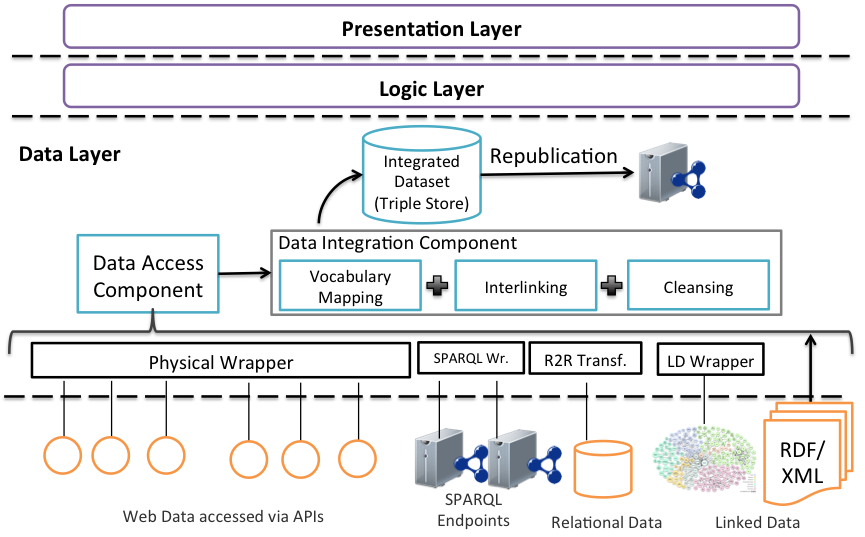
\includegraphics[width=.8\textwidth]{img/euclid_architecture.png}
	\caption{General EUCLID architecture}
	\label{euclid_architecture}
\end{figure}

The EUCLID project~\footnote{~\cite{euclid:home}} (EdUcational Curriculum for the usage of Linked Data) was founded under the \emph{Seventh Framework Program of Research and Technological Development}, a funding program of the European Union/European Commission for 2007-2013~\footnote{~\cite{eu:fp7}}\footnote{ EUCLID in the CORDIS database: \url{http://cordis.europa.eu/project/rcn/103709_en.html}}.

Aim of the project was (and still is) to gather existing knowledge and expertise of \emph{"researchers, technology enthusiasts and early adopters in various European Member States"} and provide that accumulated as educational resources to enable the  full benefit of L(O)D for European businesses. The project built upon a consortium experienced in \emph{"over 20 LD projects with over 40 companies and public offices in more than 10 countries"}~\cite{euclid:about}

The outcome of this project is a a range of learning materials, fragmented into modules, and eLearning distribution channels. Overall there are six modules:

\begin{enumerate}

	\item \textbf{Introduction and Application Scenarios}
	The introduction provides the knowledge to understand, \emph{what} Linked Data are, the main principles, the standards and the required technologies. Further, an overview how to publish and to consume the data is given.
	
	\item \textbf{Querying Linked Data}
	This chapter mainly describes SPARQL and how to use it for querying and updating.
	
	\item \textbf{Providing Linked Data}
	This module deals with the production and exposure of Linked data, using the tools as R2RML (for relational databases), Open Refine (for spreadsheets), GATECloud (for natural language) and Silk (for interlinkage between datasets, see section~\ref{silk} for details about this tool).
	
	\item \textbf{Interaction with Linked Data}
	The projects describes in this chapter, how to explore Linked Data, using visualization tools, semantic browsers and applications, introducing search options like faceted search, concept-based search and hybrid search.
	
	\item \textbf{Creating Linked Data Applications}
	This module describes how to build a Linked Data Application, which technologies to use and how to integrate common Web APIs.
	
	\item \textbf{Scaling up}
	Finally this chapter examines the main issues of scalability regarding Linked Open Data and describes the relationship to Big Data.
	
\end{enumerate}

For this thesis module 3 and 5~\footnote{~\cite{euclid:chap5}} are the most interesting. Module 3 describes some useful technologies for various steps on the way of exposing LD, but module 5 introduce a high level architecture and some patterns, how a LD application might look like (see ~\cite{euclid:chap5} for details). In detail, they provide a three-tier architecture (see figure~\ref{euclid_architecture} and three architecture patterns.

The architecture is very generic and consists of the classic three tiers: presentation, logic and data, each independent to the overlaying tier. Since the presentation and logic layer does not concern the actual publishing of the data, the data layer is the interesting one here. The layer consists of the \emph{Data Access Component}, which represents the access to different data types like relational data or other Web APIs and transforms the data to RDF, the \emph{Data Integration Component}, which does the vocabulary mapping and interlinking for the cleansing in order to e.g. identify and fix ambiguities in resource names, and finally the \emph{Triple Store}, holding the integrated dataset for exposing it to the web.

The mentioned patterns to use for implementations are:

\begin{itemize}

\item \textbf{Crawling pattern}
Used for loading the data in advance and storing them in a triple store, increasing the efficiency of data access. In exchange, the data might not be up to date when accessed.

\item \textbf{On-The-Fly Dereferencing Pattern}
Meaning that the URIs are dereferenced when the application need to access the data. This pattern provides up to date data but for the cost of performance when dereferencing many URIs.

\item \textbf{(Federated) Query Pattern}
Describing the use of complex queries on a fix set of data sources, enabling to work with current data directly retrieved from the sources. The pattern offers an access up-to-date data with adequate response time in specific situations but for the cost of the complex problem to find optimal queries.
\end{itemize}

\newacronym{lucero}{LUCERO}{Linking University Content for Education and Research Online}
\subsection{LUCERO}\index{Architectures!LUCERO}

%\begin{figure}[htbp]
%	\centering
%
\includegraphics[width=0.15\textwidth]{img/lucero_logo.png}
%\end{figure}

\begin{figure}[htbp]
	\centering
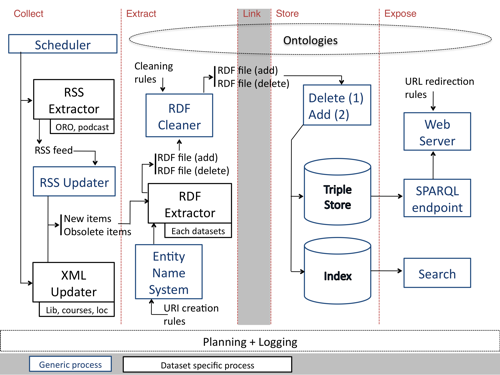
\includegraphics[width=\textwidth]{img/lucero_architecture.png}
	\caption{LUCERO work flow \& architecture}
	\label{lucero_architecture}
\end{figure}

The LUCERO project ("Linking University Content for Education and Research Online")~\footnote{The code is available in the Google Code Archive: \url{https://code.google.com/archive/p/luceroproject/wikis/StepByStepDocumentation.wiki}} was a project at the Open University, aiming to \emph{"scope, prototype, pilot and evaluate reusable, cost-effective solutions relying on the linked dataprinciples and technologies for exposing and connecting educational and research content"}. It was founded for one year by the JISC Information Environment 2011 Program under the call Deposit of research outputs and Exposing digital content for education and research.~\cite{lucero:about}

The projects connected with other organizations through LinkedUniversities.org~\footnote{\url{http://linkeduniversities.org/}} to gather common issues and practices. The outcome was the first university linked data platform,~\url{http://data.open.ac.uk/}, with a lot of impact on The Open University and the education community.

Looking at the architecture in figure~\ref{lucero_architecture} comparing to the Euclid architecture seen in the previous section, there are quite a lot of similarities. Both have components for accessing different kinds of data, here called \emph{Extractors}, for cleaning the data, here called \emph{Cleaner}, and a Triple Store, holding the data available. The lanes "Collect", "Extract", "Link" and "Store" can be seen as the data layer from the classic three-tier architecture, the "Expose" lane as the logic and presentation layer. 

Both using the crawling pattern to extract, map and store the data in a Linked Data format instead of transforming them for every request.

\subsubsection{TABLOID}\index{Tools!TABLOID}
One of the outcomes next to the LOD application itself was the Tabloid ("Toolkit ABout Linked Open Institutional Data"), \emph{"a toolkit intended to help institutions and developers to both publish and consume linked data"}. It contains work-flows, documentations, examples and tools~\cite{lucero:tabloid} trying to address different roles such as managers, developers and users. Tabloid tries to help people to understand LD, what can be done with it and gives advice on a technical perspective, how to publish and consume LD, providing at the same time a detailed and generic way.

\subsection{Linked Data book}\index{Architectures!Linked Data Book}

\begin{figure}[htbp]
	\centering
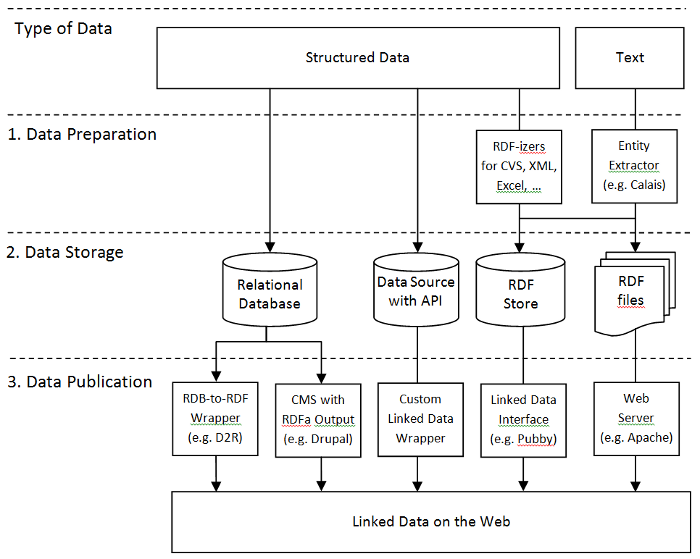
\includegraphics[width=\textwidth]{img/ld_architecture.png}
	\caption{Linked Data Publishing Options and Workflow according to the LD book}
	\label{ld_architecture}
\end{figure}

Another big effort among many others of describing LD in general, how to publish and consume them and how to implement applications, was done by the book \emph{"Linked Data: Evolving the Web into a Global Data Space"} by Heath and Bizer~\cite{heath2011linked}, which received a lot of attention.

The book aims in general to give a basic understanding of LD and describing publication and consumption of LD. They providing advices and best practices, including architectures approaches, identifying the right set of URIs and vocabulary and much more. They also described an architecture, to be seen in figure~\ref{ld_architecture}

Next to patterns they also provide a general workflow for LD publishing, see figure~\ref{ld_architecture}. But comparing to the introduced architectures in the previous sections, the workflow has a different approach: instead of holding the data in a Triple Store, the workflow access and transforms the raw data on-the-fly for every request.

Next to this workflow, the book also provides various "recipes" for publishing LD and one of them is also to hold the data in a triple store as shown by Euclid and LUCERO. Furthermore the book provides a guide for the D2R-Server, which will be described in section~\ref{d2rq}.

\newpage
\section{Frameworks}

\subsection{D2RQ Platform}\label{d2rq}\index{Framework!D2RQ Platform}

\begin{figure}[htbp]
	\centering
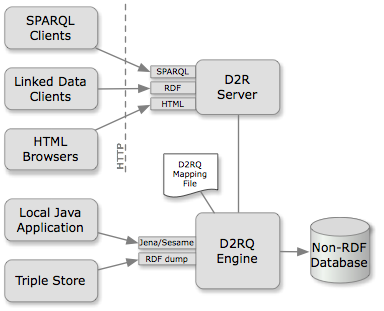
\includegraphics[width=0.8\textwidth]{img/d2rq_architecture.png}
	\caption{D2R Server architecture}
	\label{d2rq_architecture}
\end{figure}

\begin{verse}
\textbf{NOTE:} The last update on the D2RQ platform was in 2012 (version 0.8.1) and on the D2R Server in 2009 (version 0.7)
\end{verse}

The D2RQ platform~\footnote{\url{http://d2rq.org}} was introduced by the Free University of Berlin and provides a database-to-RDF mapping. It is licensed under the terms of the GNU General Public License. 

To map a relational database the platform provides a declarative mapping language, expressed in RDF, which is then be used to provide access to the database in the following, read-only, ways:~\cite{d2rq_w3c}

\begin{itemize}
\item \textbf{RDF dumps}
\item \textbf{RDF APIs}
\item \textbf{SPARQL endpoint} (D2R Server)
\item \textbf{Linked Data}
\item \textbf{HTML view} (D2R Server)
\end{itemize}

For an overview of the framework structure see figure~\ref{d2rq_architecture}.

\subsubsection{D2R Server}\index{Framework!D2RQ Platform!D2R Server}
Part of the platform is the D2R Server~\footnote{\url{http://d2rq.org/d2r-server}}, which provides the public access to the platform over SPARQL and HTML, publishing it to the semantic web. More concrete, the server provides a dereferencing interface, for HTTP request dereferencing, and a SPARQL interface. 

The server uses the mentioned \textbf{On-The-Fly Dereferencing Pattern} and does not provide a triple store, therefore it may be not has as good performance than tools with a triple store, although the team made a great effort to improve it.

Part of the server is also a tool which generates automatically a corresponding mapping and RDF vocabulary for an existing table structure, using table names as class names and column names as property names. The generated mapping file can then be customized.~\cite{bizer2006d2r}

The following applications are examples using D2R-Server:

\begin{itemize}
\itemsep0pt
\item DBLP Bibliography (University of Hannover)~\footnote{\url{http://dblp.uni-trier.de/}}
\item DBtune (University of London)~\footnote{\url{http://dbtune.org/}}
\item Database of the Nobel Prize~\footnote{\url{http://data.nobelprize.org/}}
\end{itemize}

\subsection{Information Workbench}\index{Framework!Information Workbench}

\begin{figure}[htbp]
	\centering
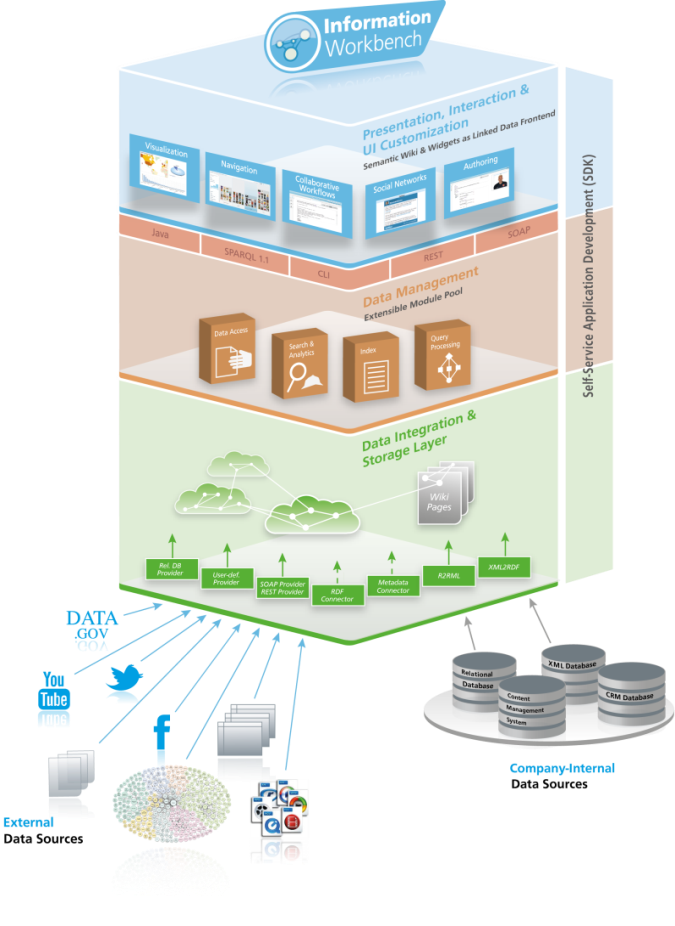
\includegraphics[width=0.9\textwidth]{img/information_workbench_architecture.png}
	\caption{Architecture of the Information Workbench}
	\label{iw_architecture}
\end{figure}

The Information Workbench~\footnote{\url{https://www.fluidops.com/en/products/information_workbench/}} is a high customizable tool to support the building of Linked Data applications, from basic data integration up to rich UI and visualization. The tool is developed by fluidOps and is published as Community Edition free available and under an Open Source License with a limited selection of capabilities and only for non-productive use (educational use, testing, development). The enterprise edition is also available but not for free.

\newpage

The workbench consists of four layers (see figure~\ref{iw_architecture} for an overview):~\cite{haase2011information}~\cite{gossenainformation}

\begin{itemize}

\item \textbf{Persistence}
Using so-called \emph{providers}, the layers offer capabilities to integrate and convert data from different data source and stores them in a central triple store. Alternatively it also supports virtualized integration of local and public Linked Data sources using a \emph{federation layer}.

\item \textbf{Platform}
On top of the persistence layer the core Platform layer a selection of modules and functionalities covering generic needs of Linked Data applications, the most important are a \emph{Semantic Wiki \& Widget Engin}e, an \emph{User Management \& Access Control}, a \emph{Search \& Analytics Engine} and a \emph{Workflow Engine}.

\item \textbf{SDK} To support customized applications the workbench provides a SDK (Solution Development Kit) for developers to build domain specific applications, including \emph{extensible data providers}, \emph{data management facilities}, modified \emph{ontologies}, \emph{templates}, \emph{widgets} and different APIs for extensive \emph{system configuration}, \emph{rules} and \emph{workflow}.

\item \textbf{Solution}
On top of all layer stands the final solution, the application itself, which is either directly deployed through a RESTful API or over a zipped file for other installation approaches.

\end{itemize}

The resulting application is again customizable by widgets and different views, enabling data exploration and visualization.

\subsection{LDIF – Linked Data Integration Framework}\index{Framework!LDIF}\newacronym{ldif}{LDIF}{Linked Data Integration Framework}

\begin{figure}[htbp]
	\centering
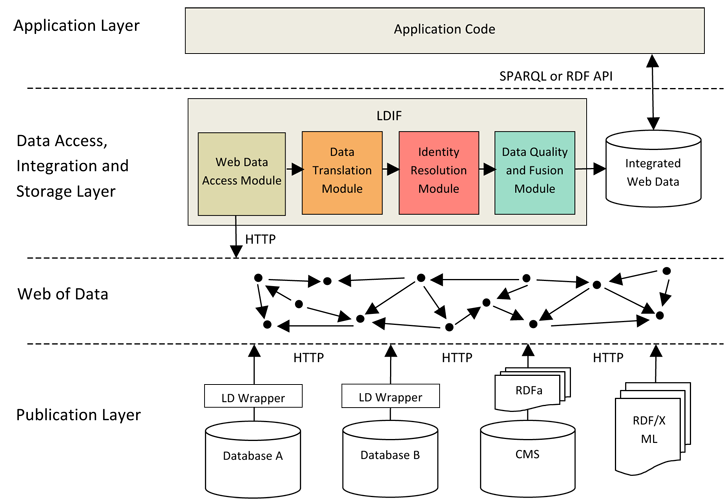
\includegraphics[width=\textwidth]{img/ldif_context.png}
	\caption{LDIF in the context of a LD application}
	\label{ldif_context}
\end{figure}

\begin{figure}[htbp]
	\centering
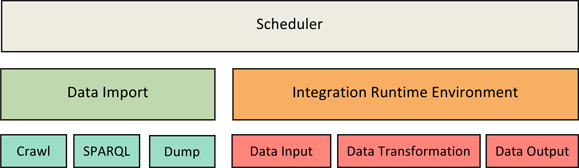
\includegraphics[width=0.8\textwidth]{img/ldif_components.png}
	\caption{Components of LDIF}
	\label{ldif_components}
\end{figure}


LDIF~\footnote{\url{http://ldif.wbsg.de/}} was developed by the University of Mannheim and is published under the terms of the Apache Software License. It is implemented in Scala and aims to translate \emph{"heterogeneous Linked Data from the Web into a clean, local target representation while keeping track of data provenance."}.

From a component perspective, LDIF consists of pluggable modules and a runtime environment, managing the data flows between them. The modules are:~\cite{schultz2011ldif}~\cite{schultz2012ldif}

\begin{itemize}

\item \textbf{Data Access Modules \& Scheduler}
For accessing the data to transform, LDIF provides several ways to import them. These import jobs are managed by a scheduler, which frequently fills a local cache. The module supports Triple/Quade Dump (for RDF/XML, N-Triples, N-Quads and Turtle formats), Crawler (using LDSpider~\footnote{\url{https://github.com/ldspider/ldspider}}) and SPARQL imports.

\item \textbf{Data Translation}
For translating Web data using different vocabularies into a single target vocabulary, LDIF uses the R2R Mapping Language~\footnote{\url{http://wifo5-03.informatik.uni-mannheim.de/bizer/r2r/spec/}}.

\item \textbf{Identity Resolution}
To find different URIs in different data pointing to the same entity, LDIF employs the Silk Link Discovery Framework with the Silk - Link Specification Language (Silk-LSL).

\item \textbf{Data Quality Assessment and Fusion}
For quality assessment, LDIF uses the Sieve Data Quality Assessment and Data Fusion Framework~\footnote{\url{http://wifo5-03.informatik.uni-mannheim.de/bizer/sieve/}}.

\item \textbf{Data Output}
In the final step, LDIF write the cleaned data together with the provenance information in a single N-Quads file or without the meta-information in a N-Triples file.
\item \textbf{Runtime Environment} 
As mentioned, the runtime environment manage the data flow between each module, providing an in-memory (fast, but limited scalable), a RDF store (using Apache Jena TDB and SPARQL queries, better scalable for the price of performance) and an Hadoop version.

\end{itemize}

\subsubsection{Silk}\index{Framework!Silk}\label{silk}
Silk~\footnote{\url{http://silkframework.org/}} is \emph{"an open source framework for integrating heterogeneous data sources."} using the declarative Silk - Link Specification Language (Silk-LSL). It generates RDF links between data sets by custom link specifications. There are three different variations:~\cite{isele2010silk}

\begin{itemize}
\item \textbf{Silk Single Machine} generates RDF links between two data items on a single machine.
\item \textbf{Silk MapReduce} is for big scale datasets, using Hadoop and distributes to multiple machines.
\item \textbf{Silk Server} is intended be used as an identity resolution component of as Linked Data consuming application. It provides a REST interface and runs as an HTTP server.
\end{itemize}

For details about the Link Discovery Framework see~\cite{volz2009silk} and~\cite{jentzsch2010silk}, for the server version consult~\cite{isele2010silk}.

\subsection{Eclipse RDF4J (formerly Sesame)}
Eclipse RDF4J~\footnote{\url{http://rdf4j.org/}} (formerly known as Sesame) is \emph{a powerful Java framework for processing and handling RDF data. This includes creating, parsing, scalable storage, reasoning and querying with RDF and Linked Data. It offers an easy-to-use API that can be connected to all leading RDF database solutions.} It can be used as an embedded part of an application or as a stand-alone server.

Originally developed as Sesame by Aduna as part of the "On-To-Knowledge" project (1999-2002), it was official forked into RDF4J. It is licensed under a BSD-style license.

The framework comes with many components, like Alibaba, an API for mapping Java classes onto ontologies. The RDF database API is unlikely similar solutions, it consists of stackable interfaces for adding functionality. Next to the intern abstract storage engine (SAIL, Storage and Inference Layer), many other triplestores are supported, like  Ontotext GraphDB, Mulgara, and AllegroGraph

\subsection{Apache Jena}

Apache Jena~\footnote{\url{https://jena.apache.org/}} is \emph{a free and open source Java framework for building Semantic Web and Linked Data applications}. It was originally developed by HP Laboratories and now maintained by the Apache Software Foundation and is licensed under the Apache License 2.0.

The framework provides an API to extract data from and write to RDF, supporting relational databases, RDF/XML, Turtle and Notation 3. In contrast to RDF4J it also supports OWL.

More concrete, Jena can be used to manipulate RDF data, storing them in a triple store and publish it as a SPARQL access point. This HTTP interface is called \emph{Fuseki}, which is in fact a sub-project of Jena and can be also run as stand-alone server using the Jetty web server.

\newpage
\section{Excluded Tools And Projects}\label{excluded}

\subsection{LD-Patterns}\index{Framework!LD-Patterns}
The Linked Data Patterns book by Dodds and Davis (see~\cite{dodds2011linked}) tried to give an overview of existing design pattern regarding LD. But they don't give concrete architectures or architecture relating information, so this thesis will not use its content. But it is suggested, that this design pattern catalogue is used additionally when creating an application.

\subsection{LOD2 Stack}\index{Tools!LOD2 Stack}

The LOD2 stack, introduced by Auer et. al., is \emph{is an integrated distribution of aligned tools which support the whole life cycle of Linked Data from extraction, authoring/creation via enrichment, interlinking, fusing to maintenance.}~\cite{auer2012managing} For this thesis the proposed stack of technology was too generic to compare it with other frameworks and the website of the project~\footnote{\url{http://stack.linkeddata.org/lod2//}} was at point of writing this thesis offline, therefore it was excluded of this thesis.

\subsection{LODUM}\index{Other LOD Projects!LODUM}

Another interesting project is the LODUM project (Linked Open Data University of Münster), the Open Data initiative of the university, hosted at the Institute for Geoinformatics' Semantic Interoperability Lab (MUSIL). The project team has co-initiated both LinkedUniversities.org and LinkedScience.org.

It was excluded for this thesis because the project don't provide public documentation of their architecture or any other part of their technical details
\url{http://lodum.de/}

\subsection{Synth and SHDM}\index{Framework!Synth}

\begin{figure}[htbp]
	\centering
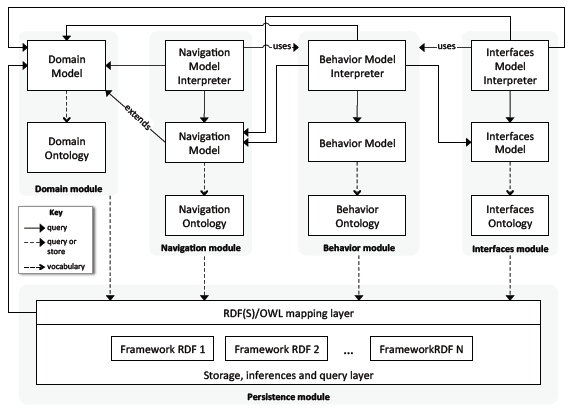
\includegraphics[width=\textwidth]{img/synth-concept.png}
	\caption{Concept of the Synth Architecture}
	\label{synth_concept}
\end{figure}

Synth~\footnote{\url{http://www.tecweb.inf.puc-rio.br/synth}} is a development environment for building SHDM~\footnote{\url{https://www.w3.org/2005/Incubator/model-based-ui/wiki/SHDM_-_Semantic_Hypermedia_Design_Method}} (Semantic Hypermedia Design Method) modeled applications, providing a set of modules, receiving SHDM generated models. Synth comes with a web browser GUI for adding and editing these models. A conceptual view of the architecture can be seen in figure~\ref{synth_concept}, where the dashed boxes are modules and the whites boxes insides the module components.~\cite{desynth} The authors de Souza Bomfim and Schwabe describe in two papers, how a Linked Data application can be build with the environment: ~\cite{desynth} and~\cite{de2011design}.

Since their description is very abstract and there are no further documentations of the tool, it was excluded for this thesis. 